\section{従来手法を用いた足動作検知実験}
この節では2015年4月から2016年10月まで取り組んでいた
従来手法の枠組みによって構築した足動作検知のBCIについて説明する。
\subsection{利用したEEGについて}
データとして被験者が8秒間静止と
8秒間足動作を8回繰り返したときに計測されたEEGを用い、
被験者はリラックスできる椅子に着席した状態で前方に配置されたディスプレイの
指示に従って動作を行った(図\ref{fig:asibumi})。
EEGの計測機器としてはg.tec社のg.USBamp\ref{fig:usbamp}を用い、ウェット式の電極を採用した。
また利用するすべての電極に関して電極インピーダンスが\(5k\Omega\)
以下になったことを確認し計測を行った。
\begin{figure}
    \centering
    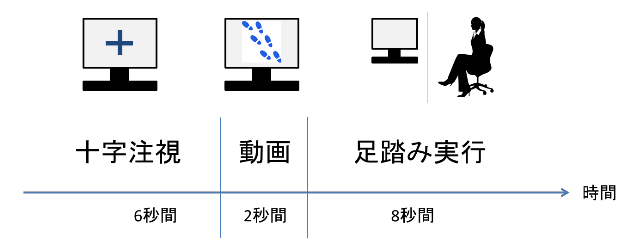
\includegraphics[width=13cm]{images/asibumi.png}
    \caption{EEG計測時のタイムスケジュール}
    \label{fig:asibumi}
\end{figure}
\begin{figure}
    \centering
    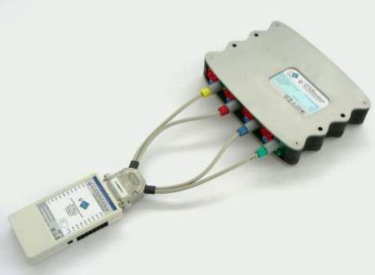
\includegraphics[width=8cm]{images/usbamp.png}
    \caption{g.tec社のg.USBamp}
    \label{fig:usbamp}
\end{figure}
